\documentclass[aspectratio=169]{beamer}
\usetheme{Madrid}
\usecolortheme{beaver}
\usepackage[utf8]{inputenc}
\usepackage[T1]{fontenc}
\usepackage{tikz}
\usepackage{amssymb}
\usepackage{graphicx}
\setbeamertemplate{navigation symbols}{}
\setbeamercolor{title}{fg=white,bg=cyan!60!black}
\setbeamercolor{frametitle}{fg=white,bg=cyan!50!black}
\setbeamercolor{block title}{bg=cyan!15,fg=black}
\setbeamercolor{block body}{bg=cyan!5,fg=black}

\title{G8 — Smart NPCs}
\subtitle{Enemies that chase, flee, patrol; a rule-based chatbot}
\author{ByteForge --- Grade 7 --- Game Maker --- Week Overview}
\date{}

\begin{document}

\begin{frame}
    \titlepage
\end{frame}

\begin{frame}{This Week's Plan}
    \begin{itemize}
        \item Lesson 1: Chase the Player
        \item Lesson 2: Patrol Pattern
        \item Lesson 3: Rule-Based Chatbot
        \item[$\bigstar$] BOSS --- Enemy with 3 Behaviours (\texttt{lessonBoss.tex})
    \end{itemize}
\end{frame}

\begin{frame}{Real-World Example}
    \Large
    An automated customer-service chat that only understands exact phrases ("Track my order") and fails on anything slightly different is a real rule-based chatbot, exactly like this chapter's. Minecraft mobs are the clearest real-world version of this whole chapter: zombies chase within a distance (chase), iron golems patrol villages, and a chatbot-style villager only "understands" exact trade offers — all rules, no learning.
\end{frame}


\begin{frame}{Image}
    \begin{center}
    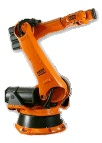
\includegraphics[width=0.55\textwidth]{../images/robot.jpg}

    \small Industrial robot — KUKA Roboter GmbH / Jo Teichmann, public domain, via Wikimedia Commons
    \end{center}
\end{frame}

\begin{frame}{Let Them Discover (1/2)}
    \Large
    Try a simple customer-service chatbot online (a bank, a shop) and type something slightly unusual. Does it understand, or does it fail and repeat a canned response? What does that tell you about how it's built?
\end{frame}


\begin{frame}{Let Them Discover (2/2)}
    \Large
    Watch a Minecraft zombie or spider from a safe distance, then get close. At roughly what distance does it notice and start chasing? That switch is exactly this chapter's distance-based if/else-if/else.
\end{frame}

\begin{frame}{Files in This Folder}
    \small
    \begin{itemize}
        \item \texttt{lesson1.tex} --- Chase the Player
        \item \texttt{lesson2.tex} --- Patrol Pattern
        \item \texttt{lesson3.tex} --- Rule-Based Chatbot
        \item \texttt{lessonBoss.tex} --- BOSS: Enemy with 3 Behaviours
    \end{itemize}
    \vspace{0.5em}
    \normalsize Each lesson file is its own short deck --- open the one for
    the specific day you're teaching, not this whole overview.
\end{frame}

\end{document}
